\documentclass[a4paper, 11pt]{article}
\usepackage[utf8]{inputenc}
  \usepackage[pdftex]{graphicx}     

%opening
\title{Protokoll Chat für Schwerhörige}
\author{René Pöcher, René Hollander}

\begin{document}

\maketitle

\newpage  \tableofcontents \newpage

\section{Aufgabenstellung}



Als 

\textbf{S04: Chat für Schwerhörige}
\\\\
Aufgabe für 2 Personen
\\\\
Erstellt ein einfaches Chat-Programm für "Schwerhörige", mit dem Texte zwischen zwei Computern geschickt werden können.
\\\\
Dabei soll jeder gesendete Text "geschrien" ankommen (d.h. ausschließlich in Großbuchstaben, lächelnd wird zu *lol*, Buchstaben werden verdoppelt, … - ihr dürft da kreativ sein)
\\\\
Zusätzlich sollen "böse" Wörter ausgefiltert und durch "\$\%\&*" ersetzt werden. Diese Funktionalität soll aber im Interface jederzeit aktiviert und deaktiviert werden können.
\\\\
Verwende dafür ausgiebig das Decorator-Pattern.

 \newpage


\section{Designüberlegung}

1) Verwenden Sie das Decorator-Pattern:
\\\\
Das Message Objekt wird als Core verwende.
Die verschiedenen Zusatzfunktionen werden in den Decorator Klassen implementiert. So können Zusatzfunktionen jederzeit ausgetauscht, abgeschaltet oder hinzugefügt werden
\\\\\\
2) Das Chatprinzip
\\\\
Der Nickname wird mittels Ip ausgelesen, so können die verschiedenen Clients sich von einander unterscheiden.

\section{Zeitaufstellung}

\subsection{Zeitschätzung}
180 Minuten Implementieren und Kommentieren pro Person
45 Minuten Testen pro Person
30 Minuten Protokoll pro Person

\subsection{Zeitaufzeichnung}

\begin{tabular}{|l|c|r|}
  \hline
  Rene Hollander & Implementation GUI 2 & 30 Minuten\\
  \hline
  Rene Hollander & Implementation ChatClient & 60 Minuten \\
  \hline
  Rene Hollander & Testen und Javadoc vervollständigen & 45 Minuten \\
  \hline
  Rene Hollander & Erste Version des Protokoll & 20 Minuten \\
  
    \hline
    Rene Pöcher &  Dekorator designen & 30 Minuten\\
    \hline
    Rene Pöcher & Implementation Message/MessageDecorator & 65 Minuten \\
    \hline
    Rene Pöcher & Zusätzliche Dekorator Funktionen überlegen plus implementieren & 30 Minuten \\
    \hline
    Rene Pöcher & Dokumentieren und finales Protokoll & 15 Minuten \\
    \hline
 \end{tabular}

\section{UML}
\subsection{UML}
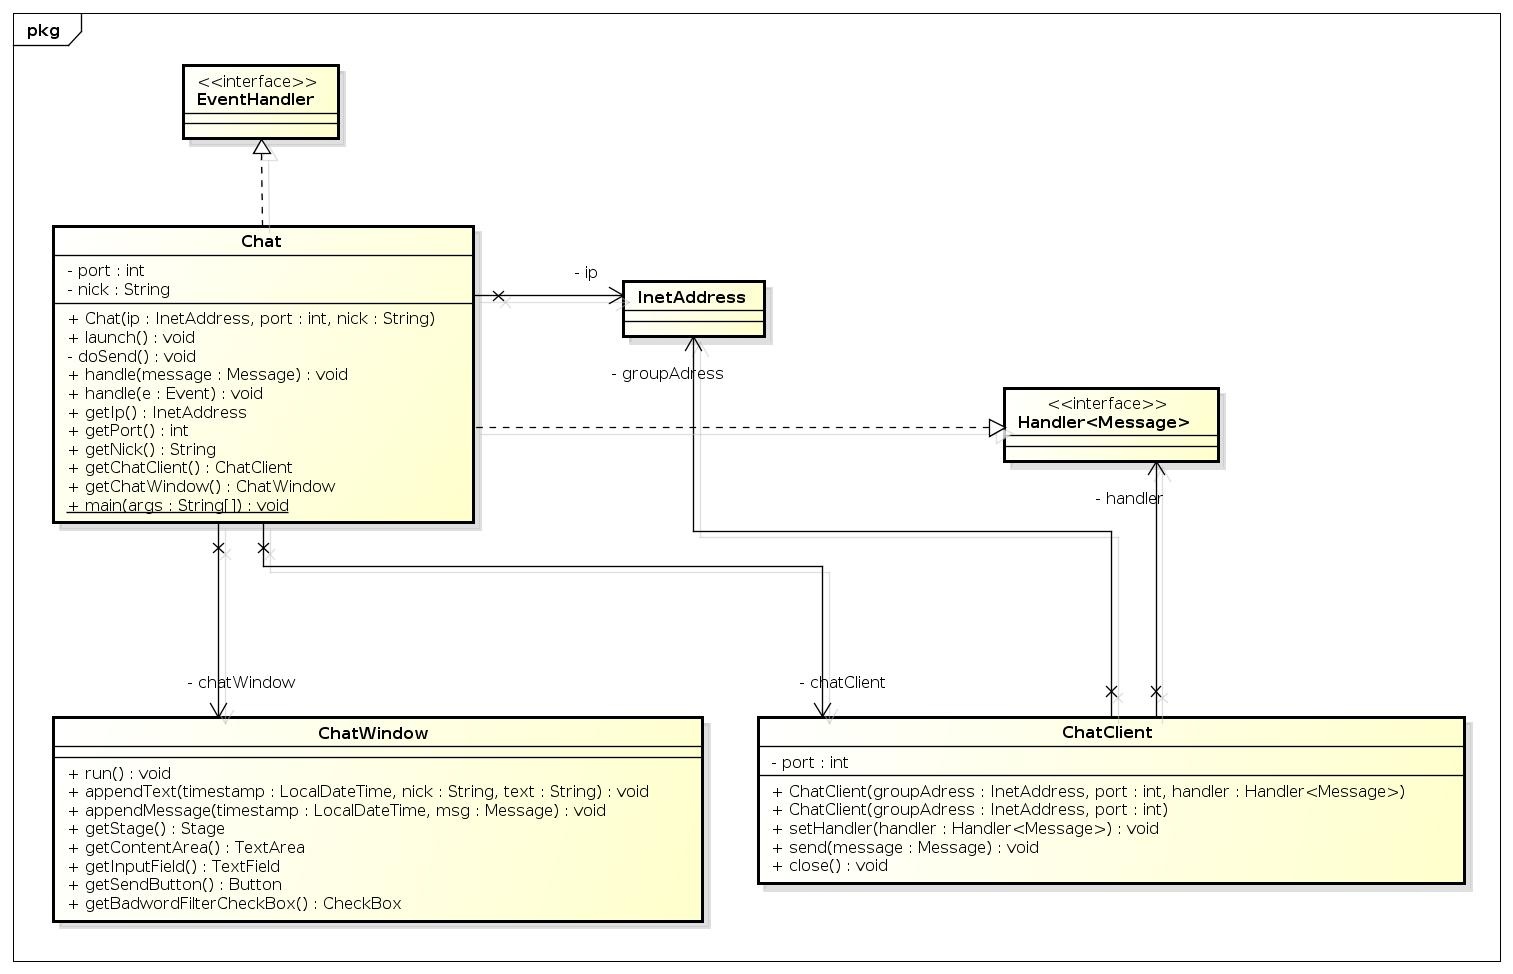
\includegraphics[width=15.5cm]{UML}

\newpage
\subsection{UML-Decorators}
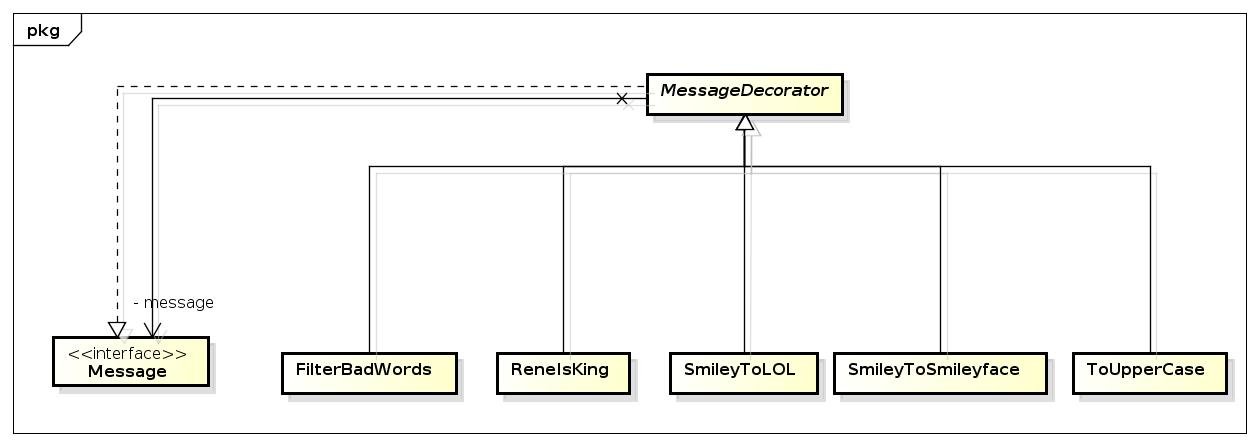
\includegraphics[width=15.5cm]{Decorators}


\section{Arbeitsdurchführung/Lessons Learned}

Für eine schnelle Programmierung ist es am besten die verschiedenen Funktionen herauszusuchen und dementsprechend zu verlinken.
So müssen nicht alle Programmteile selber programmiert/designet werden.



\section{Quellen}
[1] ReplaceAll Funktion \\
Link: http://stackoverflow.com/a/16574312 \\
Zuletzt abgerufen am: 20.11.2014 \\

\end{document}}